%% -------------------------------------
%%
%% LaTex template for academic writings of the Faculty of Engineering of the University of Buenos Aires.
%% Can be used for:
%% 	- Capstone Project (TP Profesional) / Undergraduate Thesis 
%%	- Graduate Thesis
%%	- PhD Dissertation
%%
%% Based on the mitthesis class.
%% 
%% ---------------------
%% References:
%% - Covers: https://fi.uba.ar/institucional/secretarias/secretaria-de-coordinacion-general/direccion-de-comunicacion-institucional/caratulas-de-tesis
%% - MIT Thesis class: https://web.mit.edu/thesis/tex/ - https://ctan.org/pkg/mitthesis
%%
%% ---------------------
%% Change log:
%% 	2026-03-15 - initial version.
%%
%% ---------------------
%% Authors:
%% 	Santiago Husain Cerruti - hola dot santiago at proton dot me
%%
%% ---------------------
%% Filename: FIUBA-thesis-main.tex
%% Part of FIUBA-thesis project.
%% Copyright (c) 2026 Santiago Husain Cerruti.
%% Licensed under the MIT License.
%% See LICENSE file for full text.
%%
%% THIS WORK IS PROVIDED ON AN "AS IS" BASIS.  THE AUTHOR PROVIDES NO
%% WARRANTY WHATSOEVER, EITHER EXPRESS OR IMPLIED, REGARDING THE WORK,
%% INCLUDING WARRANTIES WITH RESPECT TO ITS MERCHANTABILITY OR FITNESS
%% FOR ANY PARTICULAR PURPOSE.
% -------------------------------------
\documentclass[12pt,singlespace,a4paper]{mitthesis}

% ---------------------------------------------------
% CONFIGURATION FILE
% Everything related to this template configuration shall be 
% handled in this file.
% ---------------------------------------------------
%% -------------------------------------
%%
%% Configuration file.
%%
%% ---------------------
%% Change log:
%% 	2026-03-15 - initial version.
%%
%% ---------------------
%% Authors:
%% 	Santiago Husain Cerruti - hola dot santiago at proton dot me
%%
%% ---------------------
%% Filename: config.tex
%% Part of FIUBA-thesis project.
%% Copyright (c) 2026 Santiago Husain Cerruti.
%% Licensed under the MIT License.
%% See LICENSE file for full text.
% -------------------------------------
% -------------------------------------------------------
% FORMAT
% -------------------------------------------------------
% Input encoding and language.
\usepackage[spanish, es-tabla]{babel}
\usepackage[utf8]{inputenc}
% Refer to p.92 of "The not so short introduction to Latex" 
% by Tobias Oetiker to understand what role have this packages.
\usepackage{lmodern}
\usepackage[T1]{fontenc}
\usepackage{textcomp}
% Set Arial font.
\usepackage[scaled]{helvet} 
\renewcommand*\familydefault{\sfdefault}

% The mitthesis template uses Letter-sized pages. We must adapt it to A4 size.
\usepackage[a4paper, left=3.5cm, right=2.5cm, top=3cm, bottom=3cm]{geometry}

% Provide a high-level, flexible interface for creating document-level commands and environments.
\usepackage{xparse}

% Makes the List of Tables (LoT) and List of Figures (LoF) appear in the Table of Contents (ToC).
% The 'nottoc' option makes the Table of Contents itself not to be listed in the ToC.
\usepackage[nottoc]{tocbibind}

% Increase number-column width in LoF/LoT to avoid overfull boxes with multi-level numbering.
%Your figure numbering like 1.1.1 was wider than the default number slot in LoF.
%Widening that slot prevents line-3 overflow in FIUBA-thesis-main.lof.
\makeatletter
\renewcommand*\l@figure{\@dottedtocline{1}{1.5em}{3.2em}}
\renewcommand*\l@table{\@dottedtocline{1}{1.5em}{3.2em}}
\makeatother

% ------------------------------------------------------------------------
% PAGE MARGINS
% ------------------------------------------------------------------------
% Change this lengths as needed. Usually it's not necessary.
% Definitions:
%	\textwidth	 	the width of the text on the page.
%	\hoffset 		the horizontal offset of the text (ie: how far the text is from the left of the page).
%	\textheight 	the height of the text on the page.
%	\voffset 		the vertical offset of the text (ie: how far the text is from the top of the page).
%
% Modify/comment this parameters according to the user preferences. 
% Adds cm to the default width (if used with hoffset, centering is not altered)
%\addtolength{\textwidth}{4cm}
% Removes cm to the margin, but keeping the aspect relation of each margin.
%\addtolength{\hoffset}{-2cm}
%\addtolength{\textheight}{4cm}
%\addtolength{\voffset}{2cm}
\setlength{\headheight}{15.1pt}
% ------------------------------------------------------------------------


% To add pictures to a page at absolute positions. Useful to set the cover image.
\usepackage{eso-pic}

% Verbatim text formatting, including headers.
\usepackage{fancyvrb}
% Boxes management.
\usepackage{fancybox}
% Headers management.
\usepackage{fancyhdr}
	% First you need to clear the default layout.
	\fancyhead{}
	\fancyfoot{}
% -------------
% Uncomment this line when using two-side mode document.
% -------------
	% \fancyhead[RE]{\rightmark}
	\fancyhead[LO]{\rightmark}
	\fancyfoot[C]{\thepage}
	% Remove decorative lines.
	\renewcommand{\headrulewidth}{0pt}
	\renewcommand{\footrulewidth}{0pt}
	\pagestyle{fancy}

% To remove the page numbers uncomment the following two lines:
%\thispagestyle{empty}
%\setcounter{savepage}{\thepage}

% Package for underlining, adding color to text, and highlighting text in color.
% Text highlighting package. It solves the 'fullbox' errors when using \colorbox{declared-color}{text}.
% It doesn't support letters with accents, so they must be included using the '\'' syntax.
% Usage: \hl{text}.
\usepackage{soul}
% Sets the 'soul' package to higlight text using color red.
\sethlcolor{red}

% -------------------------------------
% Easy quoting.
\usepackage[style=american]{csquotes}


% ------------------------------------------------------------------------
% MATHS
% ------------------------------------------------------------------------
\usepackage{amsmath,amsfonts,amsthm,amssymb,amsbsy}
% Equation numbering format by section. E.g., section x, equation y: (x.y)
\numberwithin{equation}{section}
\numberwithin{figure}{section}
\usepackage{mathtools}
% Useful for arrays of equations.
\usepackage[retainorgcmds]{IEEEtrantools}

% ------------------------------------------
% Setting Up Automatic Scaling Brackets.
% ------------------------------------------
% When you write equations with tall elements like fractions or matrices, standard parentheses ( and ) stay small and look awkward. While typing \left( and \right) fixes this, doing it every single time gets exhausting and clutters your code.
% Define custom paired delimiters
\DeclarePairedDelimiter\paren{(}{)}       % Parentheses
\DeclarePairedDelimiter\sqbrac{[}{]}      % Square brackets
\DeclarePairedDelimiter\curly{\{}{\}}     % Curly braces
\DeclarePairedDelimiter\abs{\lvert}{\rvert} % Absolute value
\DeclarePairedDelimiter\norm{\lVert}{\rVert} % Norm

% ----------------------------
% Imaginary unit.
% The international standard for mathematical typesetting (ISO 80000-2) dictates that mathematical constants—like the base of the natural logarithm ($e$), pi ($\pi$), and the imaginary unit ($i$ or $j$)—should be typeset in an upright (Roman) font to clearly distinguish them from variables. (Notice how the 'i' stands straight up when using it, making it instantly recognizable as a constant rather than a variable exponent).
% ----------------------------
\newcommand{\iu}{\mathrm{i}} % Imaginary unit for math/physics
\newcommand{\ju}{\mathrm{j}} % Imaginary unit for engineering
% ----------------------------
% Generic counter
% ----------------------------
\newcounter{hipotesis_ct}
\setcounter{hipotesis_ct}{1}

% ----------------------------
% Derivatives operators.
\usepackage{derivative}

% ----------------------------
% Set operators.
% ----------------------------
% We create a dummy command \given that we will redefine inside our \set command
\providecommand\given{} 
% The 'X' allows us to inject formatting inside the delimiters
\DeclarePairedDelimiterX\set[1]\{\}{
	% This makes \given print a vertical bar that scales with the outer braces
	\renewcommand\given{\;\delimsize\vert\;}
	#1
}

% ----------------------------
% Commands to write vectors.
% ----------------------------
\usepackage[c]{esvect}
\newcommand{\vecbf}[1]{\mathbf{#1}}


% ----------------------------
% Commands to write vectors.
% ----------------------------
\usepackage[c]{esvect} % Keep this ONLY if you actually use \vv{x} for arrows somewhere
\usepackage{bm}        % The modern bold math package

% Core semantic definitions
\newcommand{\mVec}[1]{\bm{#1}}       % Bold italic vectors (works on Greek too!)
\newcommand{\Mat}[1]{\bm{#1}}        % Matrices (often same as vectors, but good to separate semantically)
\newcommand{\quat}[1]{\mathbf{#1}}   % Quaternions (Standard is upright bold)

% Note: The \dot goes OUTSIDE the \mVec so the dots don't get bolded.
% Vector decorations
\newcommand{\vechat}[1]{\hat{\mVec{#1}}}
\newcommand{\vecunit}[1]{\breve{\mVec{#1}}}
\newcommand{\vecdot}[1]{\dot{\mVec{#1}}}      % Velocity
\newcommand{\vecddot}[1]{\ddot{\mVec{#1}}}    % Acceleration
\newcommand{\vecdddot}[1]{\dddot{\mVec{#1}}}  % Jerk
\newcommand{\vecprod}[2]{#1 \times #2}

% Quaternion operations
\newcommand{\quatComp}[2]{#1 \circ #2}	% Composition.
\newcommand{\quatConj}[1]{#1^{\ast}}	% Conjugate.
\newcommand{\quatRot}[2]{\Re(#1, #2)} 	% Rotation.
% ----------------------------
% Estimators.
% Dynamically stretches the hat to perfectly cover whatever is inside of it.
\newcommand{\estimated}[1]{\widehat{#1}}

% ----------------------------
% Command for equations definitions.
% Requires the amssymb package
\newcommand{\defineEq}{\triangleq}

% ----------------------------
% Système international d'unités
\usepackage{siunitx}

% ---------------------------------
% Automatic matrix transposition.
% ---------------------------------
% This snippet uses LaTeX3 (expl3) programming to create a highly useful new math environment called bmatrixT. In short, it automatically transposes a matrix. You type the matrix normally, and when the document compiles, the code swaps the rows and columns and wraps the result in standard square brackets (a bmatrix).
% It also works with pmatrix (parentheses) and vmatrix (vertical bars).
%
% How it works (using the bmatrixT environment as example):
%
% Capturing the Content: It uses the environ package to grab everything you type inside \begin{bmatrixT} ... \end{bmatrixT} and saves it as a single chunk of text (\BODY).
%
% Deconstructing the Matrix: It splits the input at every line break (\\) to figure out the rows.
%
% It then splits each row at every ampersand (&) to separate the individual column items.
%
% It stores every single item in a temporary property list using its coordinates (Row, Column) as a tag.
%
% Rebuilding the Matrix (The Transpose): It uses nested loops to rebuild the matrix, but it reverses the order. It loops through the columns first, and the rows second.
%
% This effectively swaps the X and Y coordinates of every item.
%
% Formatting the Output: Finally, it takes the newly swapped items, adds the & and \\ symbols back in the correct spots, and feeds the whole thing into a standard bmatrix environment.
\usepackage{environ}

\ExplSyntaxOn
% Declare variables
\int_new:N \l_marine_transpose_row_int
\int_new:N \l_marine_transpose_col_int
\seq_new:N \l_marine_transpose_rows_seq
\seq_new:N \l_marine_transpose_arow_seq
\prop_new:N \l_marine_transpose_matrix_prop
\tl_new:N \l_marine_transpose_last_tl
\tl_new:N \l_marine_transpose_body_tl

% 1. The function takes TWO arguments (:nn)
% #1 is the environment type (bmatrix, pmatrix, etc.)
% #2 is the matrix content
\cs_new_protected:Nn \marine_transpose:nn
{
	\seq_set_split:Nnn \l_marine_transpose_rows_seq { \\ } { #2 }
	\int_zero:N \l_marine_transpose_row_int
	\prop_clear:N \l_marine_transpose_matrix_prop
	\seq_map_inline:Nn \l_marine_transpose_rows_seq
	{
		\int_incr:N \l_marine_transpose_row_int
		\int_zero:N \l_marine_transpose_col_int
		\seq_set_split:Nnn \l_marine_transpose_arow_seq { & } { ##1 }
		\seq_map_inline:Nn \l_marine_transpose_arow_seq
		{
			\int_incr:N \l_marine_transpose_col_int
			\prop_put:Nxn \l_marine_transpose_matrix_prop
			{
				\int_to_arabic:n { \l_marine_transpose_row_int }
				,
				\int_to_arabic:n { \l_marine_transpose_col_int }
			}
			{ ####1 }
		}
	}
	\tl_clear:N \l_marine_transpose_body_tl
	\int_step_inline:nnnn { 1 } { 1 } { \l_marine_transpose_col_int }
	{
		\int_step_inline:nnnn { 1 } { 1 } { \l_marine_transpose_row_int }
		{
			\tl_put_right:Nx \l_marine_transpose_body_tl
			{
				\prop_item:Nn \l_marine_transpose_matrix_prop { ####1,##1 }
				\int_compare:nF { ####1 = \l_marine_transpose_row_int } { & }
			}
		}
		\tl_put_right:Nn \l_marine_transpose_body_tl { \\ }
	}
	
	% 2. Wrap the output in the environment specified by #1
	\begin{#1}
		\l_marine_transpose_body_tl
	\end{#1}
}

% 3. Generate a variant that expands the second argument (nV)
\cs_generate_variant:Nn \marine_transpose:nn { nV }
\cs_generate_variant:Nn \prop_put:Nnn { Nx }

% 4. Define all the specific transpose environments
\NewEnviron{bmatrixT}{ \marine_transpose:nV { bmatrix } \BODY }
\NewEnviron{pmatrixT}{ \marine_transpose:nV { pmatrix } \BODY }
\NewEnviron{vmatrixT}{ \marine_transpose:nV { vmatrix } \BODY }
\NewEnviron{BmatrixT}{ \marine_transpose:nV { Bmatrix } \BODY } % Braces {}
\NewEnviron{VmatrixT}{ \marine_transpose:nV { Vmatrix } \BODY } % Double bars ||

\ExplSyntaxOff

% ---------------------------------------------------
% GRAPHICS AND TABLES.
% ---------------------------------------------------
% Package for improving the interface with floating objects, such as graphics.
\usepackage{float}
\usepackage{graphicx}
% Packages that offer greater flexibility when using captions for figures, etc.
\usepackage{caption}
\usepackage{subcaption}
\usepackage{epstopdf}
% -----------------------
\usepackage{booktabs}
\usepackage{multirow}

% ---------------------------------------------------
% BIBLIOGRAPHY AND APPENDICES.
% ---------------------------------------------------
% The Backend: biblatex works best with a sorting engine called biber. Explicitly stating backend=biber prevents LaTeX from accidentally trying to use older, broken engines.
\usepackage[
	backend=biber,
	style=ieee,       	% Pick your citation style (numeric, apa, ieee, authoryear)
	maxbibnames=99,   	% Usually, you want all authors in the final list...
	minbibnames=1,  	% Ensures no conflict in the bibliography
	maxcitenames=2,   	% ...but only 1 or 2 authors when citing inline
	mincitenames=1,
	uniquelist=false
]{biblatex}

% Use 'family-given' instead of 'last-first' which is technically deprecated in modern LaTeX to avoid hidden warnings.
\DeclareNameAlias{sortname}{family-given}
\DeclareNameAlias{default}{family-given}

% \adddot ensures the period is handled correctly.
\DefineBibliographyStrings{spanish}{%
	andothers = {et al\adddot},
}

% The .bib file to be used
\addbibresource{back-matter-bibliography.bib}
% Add a bibliography-only line-breaking relaxation to avoid overflow caused by a long bibliography line.
% \sloppy at bibliography start gives TeX more flexibility to break those long entries cleanly.
\AtBeginBibliography{\sloppy}

% ---------------------------------------------------
% GLOSSARY / ACRONYMS
% ---------------------------------------------------

% --------------------------------
% Spanish localization bug fix.
% Glossaries pulls in datatool, and the TeX setup only has English datatool locale files installed. With babel set to spanish, tracklang warns that no Spanish datatool locale exists. Disabling datatool locale warnings suppresses this specific non-fatal warning cleanly.
% Currently can’t install an official Spanish datatool locale, because TeX Live doesn’t ship one. datatool provides base locale files plus datatool-english and some region files, but no datatool-spanish file. The warning comes from datatool locale detection (via tracklang) when using babel with spanish.
% Alternative solution: create a custom local Spanish datatool .ldf in the project so we can remove lang-warn=false.
% Loading datatool-base with lang-warn=false disables Spanish locale warnings before glossaries triggers them.
% Use this: \usepackage[lang-warn=false]{datatool-base}
% Or this: \PassOptionsToPackage{lang-warn=false}{datatool-base}
% --------------------------------
% Required for the aligned glossary style
\usepackage{longtable}
% The 'acronym' option creates a dedicated list. The 'toc' option includes the glossary in the TOC.
\usepackage[toc,acronym,nomain,nonumberlist]{glossaries}
% No external programs needed to sort the entries. 
\makenoidxglossaries

% Force the acronyms to be bold.
\renewcommand{\glsnamefont}[1]{\textbf{#1}}

% The acronyms definitions will be aligned, and not printed like a standard dictionary (jagged text).
% Create a Custom "Flush Left" Style.
% Tweak the text width parameter 'p{0.XX\textwidth}' accordingly. It tells the second column (the acronyms descriptions) to take up XX% of the page width and wrap nicely like a normal paragraph.
% 1. Define your custom strictly left-justified style
\newglossarystyle{flushleft}{%
	\setglossarystyle{long}% Base it on the existing 'long' style
	\renewenvironment{theglossary}%
	{\begin{longtable}{@{} l p{0.85\textwidth} @{}}}
		{\end{longtable}}%
}
% 2. Tell the package to use the new style
\setglossarystyle{flushleft}

% Load the definitions here in the preamble (not in the document).
%% -------------------------------------
%%
%% Acronyms page file.
%%
%% ---------------------
%% Change log:
%% 	2026-03-15 - initial version.
%%
%% ---------------------
%% Authors:
%% 	Santiago Husain Cerruti - hola dot santiago at proton dot me
%%
%% ---------------------
%% Filename: front-matter-glossary.tex
%% Part of FIUBA-thesis project.
%% Copyright (c) 2026 Santiago Husain Cerruti.
%% Licensed under the MIT License.
%% See LICENSE file for full text.
% -------------------------------------
\newacronym{utc}{UTC}{Coordinated Universal Time}
\newacronym{adt}{ADT}{Atlantic Daylight Time}
\newacronym{est}{EST}{Eastern Standard Time}
\newacronym{SLR}{SLR}{Satellite Laser Ranging}
\newacronym{GPS}{GPS}{Global Positioning System}
\newacronym{IAU}{IAU}{International Astronomical Union}
\newacronym{FK5}{FK5}{Fundamental Katalog}
\newacronym{ECI}{ECI}{Earth-centered inertial}
\newacronym{ITRF}{ITRF}{International Terrestrial Reference Frame}
\newacronym{ECEF}{ECEF}{Earth-centered Earth-fixed}
\newacronym{IERS}{IERS}{International Earth Rotatation Service}
\newacronym{IRM}{IRM}{IERS Reference Meridian}
\newacronym{IRP}{IRP}{International Reference Pole}
\newacronym{CEP}{CEP}{Celestial Ephemeris Pole}
\newacronym{MOD}{MOD}{Mean Equinox of Date}
\newacronym{TOD}{TOD}{True Equator of Date}
\newacronym{GAST}{GAST}{Greenwich Apparent Sidereal Time}
\newacronym{MST}{MST}{Mean Solar Time}
\newacronym{UT}{UT}{Universal Time}
\newacronym{NASA}{NASA}{National Aeronautics and Space Administration}
\newacronym{JPL}{JPL}{Jet Propulsion Laboratory}
\newacronym{SFU}{SFU}{Solar Flux Unit}
\newacronym{NOAA}{NOAA}{National Oceanic and Atmospheric Administration}
\newacronym{EAM}{EAM}{Exponential Atmospheric Model}
\newacronym{SAM}{SAM}{Standard Atmosphere Model}
\newacronym{HP}{HP}{Harris-Priester}
\newacronym{SRP}{SRP}{Solar Radiation Pressure}
\newacronym{LOS}{LOS}{Line-of-Sight}
\newacronym{BC}{BC}{Ballistic Coefficient}
\newacronym{FEUV}{F \textsubscript{EUV}}{Extreme Ultraviolet Radiation}
\newacronym{EGM-96}{EGM-96}{Earth Gravity Model 1996}
\newacronym{TDRSS}{TDRSS}{NASA's Tracking and Data Relay Satellite System}
\newacronym{COTS}{COTS}{Commercial Off-The-Shelf}
\newacronym{TG}{TG}{Trajectory generator}
\newacronym{GT}{GT}{Generador de trayectorias}
\newacronym{CONAE}{CONAE}{Comisión Nacional de Actividades Espaciales}
\newacronym{POE}{POE}{Precise Orbit Ephemeris}
\newacronym{STK}{STK}{Systems Tool Kit}
\newacronym{HPOP}{HPOP}{High Precision Orbit Propagator}
\newacronym{AROM}{AROM}{Autonomous Reconfiguration and Orbit Maintenance}
\newacronym{SAR}{SAR}{Synthetic-Aperture Radar}
\newacronym{MOE}{MOE}{Mean Orbital Elements}
\newacronym{ROE}{ROE}{Relative Orbital Elements}
\newacronym{OE}{OE}{Orbital Elements}
\newacronym{SAOCOM}{SAOCOM}{Satélite Argentino de Observación Con Microondas}
\newacronym{LEO}{LEO}{Low-Earth Orbit}
\newacronym{DSS}{DSS}{Distributed Satellite Systems}
\newacronym{GNC}{GNC}{Guiado, Navegación y Control}
\newacronym{TCP}{TCP}{Transmission Control Protocol}
\newacronym{UDP}{UDP}{User Datagram Protocol}
\newacronym{XML}{XML}{Extensible Markup Language}
\newacronym{CSV}{CSV}{Comma-Separated Values}
\newacronym{YAML}{YAML}{YAML Ain't Markup Language}
\newacronym{RF}{RF}{Radiofrequencia}
\newacronym{CAN}{CAN}{Controller Area Network}
\newacronym{MVC}{MVC}{Model-View-Controller}
\newacronym{OP}{OP}{Observer Pattern}
\newacronym{ENP}{ENP}{Event Notification Pattern}

















	
% ---------------------------------------------------
% MISC.
% ---------------------------------------------------
% This pack­age sim­pli­fies the in­clu­sion of ex­ter­nal multi-page PDF doc­u­ments in LaTeX doc­u­ments. 
\usepackage{pdfpages}
\setboolean{@twoside}{false}

% ------------------------------------------------------------------------
% SOURCE CODE
% ------------------------------------------------------------------------
\usepackage[dvipsnames,svgnames]{xcolor} 
\usepackage{listings}
\usepackage{caption} % Better handling of code captions
% Algorithms and pseudocode handling.
\usepackage{algorithm}
\usepackage{algpseudocode}
\makeatletter
\renewcommand{\ALG@name}{Algoritmo}
\renewcommand{\listalgorithmname}{Lista de \ALG@name s}
\algrenewcommand\algorithmicensure{\textbf{Salida:}}
\algrenewcommand\algorithmicrequire{\textbf{Entrada:}}
\algnewcommand{\LineComment}[1]{\State \(\triangleright\) #1}
\makeatother

% ------------------------------------------------------------------------
% GLOBAL SETTINGS (Applied to all code)
% ------------------------------------------------------------------------
\lstset{
	inputencoding=utf8,
	extendedchars=true,
	literate={á}{{\'a}}1 {é}{{\'e}}1 {í}{{\'i}}1 {ó}{{\'o}}1 {ú}{{\'u}}1 {ñ}{{\~n}}1 {Á}{{\'A}}1 {É}{{\'E}}1 {Í}{{\'I}}1 {Ó}{{\'O}}1 {Ú}{{\'U}}1 {ü}{{\"u}}1 {Ü}{{\"U}}1,
	basicstyle=\ttfamily\small,
	breaklines=true,			% Enable wrapping
	breakatwhitespace=false,    % Wrap even if there isn't a space
	captionpos=b,
	keepspaces=true,
	showstringspaces=false,
	upquote=true,
	columns=fullflexible,       % Improves character spacing after wrapping
	postbreak=\mbox{\textcolor{red}{$\hookrightarrow$}\space} % Adds a little red arrow at the wrap point.
}

% Spanish Localization
\renewcommand{\lstlistingname}{Código fuente}       	% For the caption
\renewcommand{\lstlistlistingname}{Índice de códigos} 	% For the table of contents

% ------------------------------------------------------------------------
% DEFINE CUSTOM STYLES
% ------------------------------------------------------------------------

% 1. C/C++ Style
\lstdefinestyle{StyleC}{
	language=C++,
	commentstyle=\color{ForestGreen},
	keywordstyle=\color{RoyalBlue},
	stringstyle=\color{BrickRed},
	numberstyle=\tiny\color{gray},
	numbers=left,
	frame=lines,
	backgroundcolor=\color{gray!5}
}

% 2. YAML Style
\lstdefinelanguage{yaml}{
	keywords={true,false,null,y,n},
	keywordstyle=\color{darkgray}\bfseries,
	sensitive=false,
	comment=[l]{\#},
	morecomment=[s]{/*}{*/},
	commentstyle=\color{purple}\ttfamily,
	stringstyle=\color{blue}\ttfamily,
	moredelim=[l][\color{orange}]{\&},
	moredelim=[l][\color{magenta}]{*},
	moredelim=**[il][\color{red}{:}\color{blue}]{:},
	morestring=[b]',
	morestring=[b]",
	frame=lines,
	backgroundcolor=\color{gray!5}
}

% 3. Terminal Style (For console output)
\lstdefinestyle{terminal}{
	backgroundcolor=\color{black},
	basicstyle=\ttfamily\small\color{white},
	frame=lines,
	numbers=none
}


% ---------------------------------------------------
% WATERMARK
% Useful to produce drafts before publishing.
% ---------------------------------------------------
\usepackage{draftwatermark}
\SetWatermarkLightness{0.9}
\SetWatermarkScale{0.8}
\SetWatermarkText{BORRADOR}

% ---------------------------------------------------
% HYPERTEXT.
% WARNING: must always be the last loaded package.
% ---------------------------------------------------
% Package for using hypertext. All links, references, etc., become hypertext.
\usepackage[pdftex,breaklinks]{hyperref}
\hypersetup{
	pdfdisplaydoctitle=true,
	colorlinks=true,
	urlcolor = blue,		
	pdfnewwindow=true,
	linkcolor=blue,
	citecolor=blue,
	filecolor=blue,
	linktocpage=true,
% !!!!!!!!!!!!!!!!!!!!!!!!!!!!!!!!!
% FILL IN WITH YOUR INFORMATION
% !!!!!!!!!!!!!!!!!!!!!!!!!!!!!!!!!
	pdftitle={PDF TITLE},
	pdfauthor={PDF AUTHOR}
}

\begin{document}
\sisetup{range-phrase=--}
\sisetup{range-units = single}
% I'm removing the extra space added between paragraphs.
\raggedbottom
% The first pages are numbered in Roman numerals, followed by Arabic numerals.
\pagenumbering{roman}
% ---------------------------------------------------
% COVER PAGE
% Comment the two that do not apply to the current degree.
% ---------------------------------------------------
%\include{front-matter-cover-undergraduate-thesis.tex}
\include{front-matter-cover-graduate-thesis.tex}
%%% -------------------------------------
%%
%% PhD dissertation cover page file.
%%
%% ---------------------
%% Change log:
%% 	2026-03-15 - initial version.
%%
%% ---------------------
%% Authors:
%% 	Santiago Husain Cerruti - hola dot santiago at proton dot me
%%
%% ---------------------
%% Filename: front-matter-cover-phd-dissertation.tex
%% Part of FIUBA-thesis project.
%% Copyright (c) 2026 Santiago Husain Cerruti.
%% Licensed under the MIT License.
%% See LICENSE file for full text.
% -------------------------------------
\AddToShipoutPictureBG*{%
	
\includegraphics[width=\paperwidth,height=\paperheight]{media/front-matter-cover/03-FIUBA-phd-dissertation-cover-background.png}%
}

\begin{titlepage}
	\thispagestyle{empty}
	% 1. VERTICAL PUSH
	\vspace*{-4cm}
	% ---------------------
	% 1. HORIZONTAL PUSH
	% Add space to the left to shove the minipage to the right.
	% Adjust this value (e.g., 2cm, 4cm) to move it as far right as you want.
	\noindent\hspace*{2.5cm}%
	\begin{minipage}[t][0.9\textheight][t]{0.8\textwidth}
		\raggedleft % Re-applied Right Alignment
		
		% 1. TITLE (Grows UPWARDS from 445.5bp)
		\vspace*{445.5bp}%
		\begin{minipage}[b][0pt][b]{\linewidth}%
			\raggedleft
			{\fontsize{33}{40}\selectfont\textbf{[(Título del trabajo)]}\par}%
			% Comment the following line if there is no sub-title.
			{\fontsize{23}{40}\selectfont\textbf{[(Sub-título)]}\par}%
		\end{minipage}
		
		% 2. AUTHORS
		\vspace{36.5bp}%
		{\fontsize{20}{24}\selectfont [(Nombre del Autor)]\par}
		
		% 3. DEGREE NAME
		\vspace{20bp}% 
		{\fontsize{15}{18}\selectfont Tesis doctoral\par}
		
		% 4. DIRECTOR
		\vspace{23.3bp}%
		{\fontsize{11}{13}\selectfont Director:\par}
		{\fontsize{11}{13}\selectfont [(Nombre del Director) (afiliación)]\par}
		% Comment the following two lines if there is no co-director.
		{\fontsize{11}{13}\selectfont Co-director:\par}
		{\fontsize{11}{13}\selectfont [(Nombre del Co-Director) (afiliación)]\par}
		
		% 5. COMMITTEE
		\vspace{36.5bp}%
		{\fontsize{11}{13}\selectfont Jurados:\par}
		{\fontsize{11}{13}\selectfont [(Nombre de Jurado 1) (afiliación)]\par}
		{\fontsize{11}{13}\selectfont [(Nombre de Jurado 2) (afiliación)]\par}
		{\fontsize{11}{13}\selectfont [(Nombre de Jurado 3) (afiliación)]\par}
		{\fontsize{11}{13}\selectfont [(Nombre de Jurado 4) (afiliación)]\par}
		
		% 6. DATE AND PLACE
		\vspace{21.1bp}%
		{\fontsize{10}{12}\selectfont\textit{[Este trabajo fue realizado en (LUGAR), (DD) de (MES) de (AÑO).]}\par}
	\end{minipage}%
	% 2. HORIZONTAL PULL: Apply the EXACT SAME negative space to the right.
	% This tricks LaTeX's centering mechanism into thinking the block hasn't moved.
	\hspace*{-2.5cm}
	% ---------------------
	% 2. VERTICAL PULL: Apply the exact opposite space at the bottom.
	% Since we added 2cm at the top, we subtract 2cm here.
	\vspace*{4cm}
\end{titlepage}

% ---------------------------------------------------
% SIGNATURES PAGE
% Some departments require an additional cover page
% with signatures of the thesis committee.  Please check with your
% thesis advisor or other appropriate person to determine if such a 
% page is required for your thesis.
% ---------------------------------------------------
%% -------------------------------------
%%
%% Signatures page file.
%%
%% ---------------------
%% Change log:
%% 	2026-03-15 - initial version.
%%
%% ---------------------
%% Authors:
%% 	Santiago Husain Cerruti - hola dot santiago at proton dot me
%%
%% ---------------------
%% Filename: front-matter-signature.tex
%% Part of FIUBA-thesis project.
%% Copyright (c) 2026 Santiago Husain Cerruti.
%% Licensed under the MIT License.
%% See LICENSE file for full text.
% -------------------------------------
\begin{titlepage}
\begin{large}
\begin{flushleft}
	\textbf{Este trabajo fue producido por}
\end{flushleft}

\signature{(Nombre del autor de tesis)}{Estudiante de grado de Ing. Electrónica de FIUBA.}

\begin{flushleft}
	\textbf{Este trabajo fue dirigido por}
\end{flushleft}

\signature{(Nombre del director de tesis)}{Profesor de FIUBA.}
\signature{(Nombre del co-director de tesis)}{Puesto laboral.}

\begin{flushleft}
	\textbf{Este trabajo fue examinado por el siguiente Tribunal}
\end{flushleft}

\signature{(Nombre de Jurado 1)}{Miembro del Tribunal Examinador \\ Profesor de FIUBA.}

\signature{(Nombre de Jurado 2)}{Miembro del Tribunal Examinador \\ Profesor de FIUBA.}

\signature{(Nombre de Jurado 3)}{Miembro del Tribunal Examinador \\ Puesto laboral Jurado 3.}

\signature{(Nombre de Jurado 4)}{Miembro del Tribunal Examinador \\ Puesto laboral Jurado 4.}

Este trabajo obtuvo la siguiente calificación:

\signature{}{}
\end{large}
\end{titlepage}


% ---------------------------------------------------
% ABSTRACT PAGE
% A concise summary of the research problem, methodology, and key findings.
% ---------------------------------------------------
\begin{abstractpage}
%% -------------------------------------
%%
%% Abstract page file.
%%
%% ---------------------
%% Change log:
%% 	2026-03-15 - initial version.
%%
%% ---------------------
%% Authors:
%% 	Santiago Husain Cerruti - hola dot santiago at proton dot me
%%
%% ---------------------
%% Filename: front-matter-abstract.tex
%% Part of FIUBA-thesis project.
%% Copyright (c) 2026 Santiago Husain Cerruti.
%% Licensed under the MIT License.
%% See LICENSE file for full text.
% -------------------------------------
Lorem ipsum dolor sit amet, consectetur adipiscing elit. Quisque semper arcu vel enim consectetur, facilisis feugiat dolor bibendum. Donec commodo lacus eget elit dapibus, a venenatis felis consequat. Aliquam consectetur lectus eu dui volutpat scelerisque. Sed laoreet nisi in magna eleifend tempus. Ut ac urna nec nunc tincidunt cursus sit amet eu purus. Sed convallis gravida mi, egestas finibus felis tempus vel. Donec odio sem, laoreet eget maximus elementum, commodo in mi. Pellentesque ut placerat ante. In eu justo eget ligula bibendum molestie eget in nulla. Nam malesuada nisl orci, elementum vulputate nisl pharetra sit amet. Nulla sit amet viverra tortor, a volutpat quam. Nulla quis mauris a justo consequat gravida. Donec posuere lorem id consectetur egestas.

Nullam sed porta risus. Nulla non metus quis quam porta laoreet. Donec egestas nisl purus, a dignissim neque venenatis tempor. Proin facilisis quam eget sem vulputate ultrices. Aliquam sed enim id enim tincidunt sodales eget in enim. Nulla eget finibus libero. Fusce non tristique elit, eget varius erat. Pellentesque malesuada, nulla non rhoncus condimentum, leo nisi sagittis lacus, vel lobortis eros est pretium neque. Nulla nunc justo, convallis sed nibh sit amet, bibendum consectetur lacus.

Lorem ipsum dolor sit amet, consectetur adipiscing elit. Quisque semper arcu vel enim consectetur, facilisis feugiat dolor bibendum. Donec commodo lacus eget elit dapibus, a venenatis felis consequat. Aliquam consectetur lectus eu dui volutpat scelerisque. Sed laoreet nisi in magna eleifend tempus. Ut ac urna nec nunc tincidunt cursus sit amet eu purus. Sed convallis gravida mi, egestas finibus felis tempus vel. Donec odio sem, laoreet eget maximus elementum, commodo in mi. Pellentesque ut placerat ante. In eu justo eget ligula bibendum molestie eget in nulla. Nam malesuada nisl orci, elementum vulputate nisl pharetra sit amet. Nulla sit amet viverra tortor, a volutpat quam. Nulla quis mauris a justo consequat gravida. Donec posuere lorem id consectetur egestas.

Nullam sed porta risus. Nulla non metus quis quam porta laoreet. Donec egestas nisl purus, a dignissim neque venenatis tempor. Proin facilisis quam eget sem vulputate ultrices. Aliquam sed enim id enim tincidunt sodales eget in enim. Nulla eget finibus libero. Fusce non tristique elit, eget varius erat. Pellentesque malesuada, nulla non rhoncus condimentum, leo nisi sagittis lacus, vel lobortis eros est pretium neque. Nulla nunc justo, convallis sed nibh sit amet, bibendum consectetur lacus.

Lorem ipsum dolor sit amet, consectetur adipiscing elit. Quisque semper arcu vel enim consectetur, facilisis feugiat dolor bibendum. Donec commodo lacus eget elit dapibus, a venenatis felis consequat. Aliquam consectetur lectus eu dui volutpat scelerisque. Sed laoreet nisi in magna eleifend tempus. Ut ac urna nec nunc tincidunt cursus sit amet eu purus. Sed convallis gravida mi, egestas finibus felis tempus vel. Donec odio sem, laoreet eget maximus elementum, commodo in mi. Pellentesque ut placerat ante. In eu justo eget ligula bibendum molestie eget in nulla. Nam malesuada nisl orci, elementum vulputate nisl pharetra sit amet. Nulla sit amet viverra tortor, a volutpat quam. Nulla quis mauris a justo consequat gravida. Donec posuere lorem id consectetur egestas.
\end{abstractpage}

% ---------------------------------------------------
% ACKNOWLEDMENTS PAGE
% A space to thank those who supported your research journey.
% ---------------------------------------------------
%% -------------------------------------
%%
%% Acknowledgements page file.
%%
%% ---------------------
%% Change log:
%% 	2026-03-15 - initial version.
%%
%% ---------------------
%% Authors:
%% 	Santiago Husain Cerruti - hola dot santiago at proton dot me
%%
%% ---------------------
%% Filename: front-matter-acknowledgements.tex
%% Part of FIUBA-thesis project.
%% Copyright (c) 2026 Santiago Husain Cerruti.
%% Licensed under the MIT License.
%% See LICENSE file for full text.
% -------------------------------------
\thispagestyle{empty}
\null\vspace{\stretch {1}}
\section*{Agradecimientos}
Lorem ipsum dolor sit amet, consectetur adipiscing elit. Quisque semper arcu vel enim consectetur, facilisis feugiat dolor bibendum. Donec commodo lacus eget elit dapibus, a venenatis felis consequat. Aliquam consectetur lectus eu dui volutpat scelerisque. Sed laoreet nisi in magna eleifend tempus. Ut ac urna nec nunc tincidunt cursus sit amet eu purus. Sed convallis gravida mi, egestas finibus felis tempus vel. Donec odio sem, laoreet eget maximus elementum, commodo in mi. Pellentesque ut placerat ante. In eu justo eget ligula bibendum molestie eget in nulla. Nam malesuada nisl orci, elementum vulputate nisl pharetra sit amet. Nulla sit amet viverra tortor, a volutpat quam. Nulla quis mauris a justo consequat gravida. Donec posuere lorem id consectetur egestas.

Nullam sed porta risus. Nulla non metus quis quam porta laoreet. Donec egestas nisl purus, a dignissim neque venenatis tempor. Proin facilisis quam eget sem vulputate ultrices. Aliquam sed enim id enim tincidunt sodales eget in enim. Nulla eget finibus libero. Fusce non tristique elit, eget varius erat. Pellentesque malesuada, nulla non rhoncus condimentum, leo nisi sagittis lacus, vel lobortis eros est pretium neque. Nulla nunc justo, convallis sed nibh sit amet, bibendum consectetur lacus.

Nullam sed porta risus. Nulla non metus quis quam porta laoreet. Donec egestas nisl purus, a dignissim neque venenatis tempor. Proin facilisis quam eget sem vulputate ultrices. Aliquam sed enim id enim tincidunt sodales eget in enim. Nulla eget finibus libero. Fusce non tristique elit, eget varius erat. Pellentesque malesuada, nulla non rhoncus condimentum, leo nisi sagittis lacus, vel lobortis eros est pretium neque. Nulla nunc justo, convallis sed nibh sit amet, bibendum consectetur lacus.

Nullam sed porta risus. Nulla non metus quis quam porta laoreet. Donec egestas nisl purus, a dignissim neque venenatis tempor. Proin facilisis quam eget sem vulputate ultrices. Aliquam sed enim id enim tincidunt sodales eget in enim. Nulla eget finibus libero. Fusce non tristique elit, eget varius erat. Pellentesque malesuada, nulla non rhoncus condimentum, leo nisi sagittis lacus, vel lobortis eros est pretium neque. Nulla nunc justo, convallis sed nibh sit amet, bibendum consectetur lacus.

Lorem ipsum dolor sit amet consectetur adipiscing elit. Quisque faucibus ex sapien vitae pellentesque sem placerat. In id cursus mi pretium tellus duis convallis. Tempus leo eu aenean sed diam urna tempor. Pulvinar vivamus fringilla lacus nec metus bibendum egestas. Iaculis massa nisl malesuada lacinia integer nunc posuere. Ut hendrerit semper vel class aptent taciti sociosqu. Ad litora torquent per conubia nostra inceptos himenaeos.

Lorem ipsum dolor sit amet consectetur adipiscing elit. Quisque faucibus ex sapien vitae pellentesque sem placerat. In id cursus mi pretium tellus duis convallis. Tempus leo eu aenean sed diam urna tempor. Pulvinar vivamus fringilla lacus nec metus bibendum egestas. Iaculis massa nisl malesuada lacinia integer nunc posuere. Ut hendrerit semper vel class aptent taciti sociosqu. Ad litora torquent per conubia nostra inceptos himenaeos.
\vspace{\stretch{2}}\null

% ---------------------------------------------------
% EPIGRAPH PAGE
% A short personal note or a relevant quotation that sets the tone for the work.
% ---------------------------------------------------
%% -------------------------------------
%%
%% Epigraph page file.
%%
%% ---------------------
%% Change log:
%% 	2026-03-15 - initial version.
%%
%% ---------------------
%% Authors:
%% 	Santiago Husain Cerruti - hola dot santiago at proton dot me
%%
%% ---------------------
%% Filename: front-matter-epigraph.tex
%% Part of FIUBA-thesis project.
%% Copyright (c) 2026 Santiago Husain Cerruti.
%% Licensed under the MIT License.
%% See LICENSE file for full text.
% -------------------------------------
\thispagestyle{empty}
\null\vspace{\stretch {1}}
\begin{flushright}
	\emph{EPÍGRAFE.
		\vspace{5mm}}
\end{flushright}
\vspace{\stretch{2}}\null

% ---------------------------------------------------
% CONTENTS
\tableofcontents
\cleardoublepage

\listoffigures
\cleardoublepage

\listoftables
\cleardoublepage

% Print the glossary first! It handles its own page breaks.
\printnoidxglossary[type=\acronymtype, title={Lista de Acrónimos}]
\glsaddall
\cleardoublepage

% ---------------------------------------------------
% CHAPTERS
% ---------------------------------------------------
\pagenumbering{arabic}
\setcounter{page}{1}
%% -------------------------------------
%%
%% Introduction chapter file.
%%
%% ---------------------
%% Change log:
%% 	2026-03-15 - initial version.
%%
%% ---------------------
%% Authors:
%% 	Santiago Husain Cerruti - hola dot santiago at proton dot me
%%
%% ---------------------
%% Filename: main-body-chapter-intro.tex
%% Part of FIUBA-thesis project.
%% Copyright (c) 2026 Santiago Husain Cerruti.
%% Licensed under the MIT License.
%% See LICENSE file for full text.
% -------------------------------------
\chapter{Introducción}

\textbf{VER EL CÓDIGO LATEX DE EJEMPLO EN LOS DIFERENTES CAPÍTULOS}

Se muestra cómo:
\begin{itemize}
	\item Escribir ecuaciones
	\item Mostras figuras
	\item Definir tablas
	\item Definir y usar acrónimos
	\item Incluir snippets de código fuente y pseudocódigo.
	\item Citar referencias
\end{itemize}


\textbf{Cómo usar acrónimos}

Así se utiliza un acrónimo: \gls{CONAE}. La primera vez va a aparecer el acrónimo completo. La segunda vez solamente el acrónimo: \gls{CONAE}.




\textbf{Agrego texto aleatorio}

Lorem ipsum dolor sit amet, consectetur adipiscing elit. Quisque semper arcu vel enim consectetur, facilisis feugiat dolor bibendum. Donec commodo lacus eget elit dapibus, a venenatis felis consequat. Aliquam consectetur lectus eu dui volutpat scelerisque. Sed laoreet nisi in magna eleifend tempus. Ut ac urna nec nunc tincidunt cursus sit amet eu purus. Sed convallis gravida mi, egestas finibus felis tempus vel. Donec odio sem, laoreet eget maximus elementum, commodo in mi. Pellentesque ut placerat ante. In eu justo eget ligula bibendum molestie eget in nulla. Nam malesuada nisl orci, elementum vulputate nisl pharetra sit amet. Nulla sit amet viverra tortor, a volutpat quam. Nulla quis mauris a justo consequat gravida. Donec posuere lorem id consectetur egestas.


\section{Sección}

\textbf{Agrego texto aleatorio}

Lorem ipsum dolor sit amet, consectetur adipiscing elit. Quisque semper arcu vel enim consectetur, facilisis feugiat dolor bibendum. Donec commodo lacus eget elit dapibus, a venenatis felis consequat. Aliquam consectetur lectus eu dui volutpat scelerisque. Sed laoreet nisi in magna eleifend tempus. Ut ac urna nec nunc tincidunt cursus sit amet eu purus. Sed convallis gravida mi, egestas finibus felis tempus vel. Donec odio sem, laoreet eget maximus elementum, commodo in mi. Pellentesque ut placerat ante. In eu justo eget ligula bibendum molestie eget in nulla. Nam malesuada nisl orci, elementum vulputate nisl pharetra sit amet. Nulla sit amet viverra tortor, a volutpat quam. Nulla quis mauris a justo consequat gravida. Donec posuere lorem id consectetur egestas.

\begin{figure}[t]
	\centering
	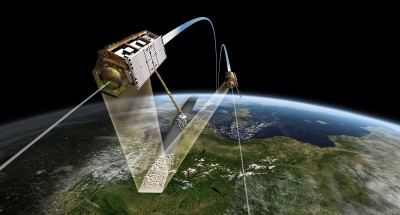
\includegraphics[scale=1]{media/main-body-chapter-intro/TandemX-wiki.jpg}
	\caption{TandemX.}\label{TandemX}
\end{figure}

\subsection{Subsección}

\begin{IEEEeqnarray}{rCl}
	\mathbf{\ddot{r}}_{SRP} & = & - \frac{p_{srp}\,C_R\,A_{srp}}{m} \, \frac{\mathbf{d}}{d} \label{eq:srp_def}
\end{IEEEeqnarray}

\begin{IEEEeqnarray}{rCl}
	A_c & = & r^2 + \norm{\vecbf{s - r}}^2\,\tau_{min}^2 + 2\,\left(\vecbf{s-r}\right)\cdot\vecbf{r}\,\tau_{min} \nonumber \\
	& = & r^2 + \left(s^2 + r^2 - 2\,\vecbf{r}\cdot\vecbf{s}\right)\,\tau_{min}^2 + 2\,\left(-r^2 + \vecbf{r}\cdot\vecbf{s} \right) \tau_{min} \nonumber \\
	& = & r^2\left(1 - 2\,\tau_{min}\right) + 2\,\vecbf{r}\cdot\vecbf{s}\,\tau_{min} + \frac{\left(r^2-\vecbf{r}\cdot\vecbf{s}\right)}{r^2+s^2-2\,\vecbf{r}\cdot\vecbf{s}} \\
	& = & r^2\left(1 - 2\,\tau_{min}\right) + 2\,\vecbf{r}\cdot\vecbf{s}\tau_{min} + \left(r^2 - \vecbf{r}\cdot\vecbf{s}\right)\,\tau_{min} \nonumber 
\end{IEEEeqnarray}

Donec egestas nisl purus, a dignissim neque venenatis tempor. Proin facilisis quam eget sem vulputate ultrices. Aliquam sed enim id enim tincidunt sodales eget in enim. Nulla eget finibus libero. Fusce non tristique elit, eget varius erat. Pellentesque malesuada, nulla non rhoncus condimentum, leo nisi sagittis lacus, vel lobortis eros est pretium neque. Nulla nunc justo, convallis sed nibh sit amet, bibendum consectetur lacus. \footnote{Nulla eget finibus libero. Fusce non tristique elit, eget varius erat. Pellentesque malesuada, nulla non rhoncus condimentum, leo nisi sagittis lacus, vel lobortis eros est pretium neque. Nulla nunc justo, convallis sed nibh sit amet, bibendum consectetur lacus.}\footnote{Nulla eget finibus libero. Fusce non tristique elit, eget varius erat. Pellentesque malesuada, nulla non rhoncus condimentum, leo nisi sagittis lacus, vel lobortis eros est pretium neque.}

Nullam sed porta risus. Nulla non metus quis quam porta laoreet. Donec egestas nisl purus, a dignissim neque venenatis tempor. Proin facilisis quam eget sem vulputate ultrices. Aliquam sed enim id enim tincidunt sodales eget in enim. Nulla eget finibus libero. Fusce non tristique elit, eget varius erat. Pellentesque malesuada, nulla non rhoncus condimentum, leo nisi sagittis lacus, vel lobortis eros est pretium neque. Nulla nunc justo, convallis sed nibh sit amet, bibendum consectetur lacus.\footnote{Nulla eget finibus libero. Fusce non tristique elit, eget varius erat. Pellentesque malesuada, nulla non rhoncus condimentum, leo nisi sagittis lacus, vel lobortis eros est pretium neque. Nulla nunc justo, convallis sed nibh sit amet, bibendum consectetur lacus.}


\begin{IEEEeqnarray}{rCl}
	\begin{bmatrix}
		\vecbf{r}(t_0) \\
		\vecbf{v}(t_0)
	\end{bmatrix}
	&=& 
	\begin{bmatrix}
		\SI{-7106.36}{\kilo\meter}  		  \\
		\SI{0}{\kilo\meter} 				  \\
		\SI{0}{\kilo\meter} 				  \\
		\SI{0}{\kilo\meter\per\second} 		  \\
		\SI{-1.04752}{\kilo\meter\per\second} \\
		\SI{7.45348}{\kilo\meter\per\second}
	\end{bmatrix} \quad \rightarrow \quad 
	\begin{bmatrix}
		a(t_0) \\
		e(t_0) \\
		i(t_0) \\
		\Omega(t_0) \\
		\omega(t_0) \\
		M(t_0)
	\end{bmatrix} = 
	\begin{bmatrix}
		\SI{7178.162}{\kilo\meter} \\
		\SI{0.01000}{} \\
		\SI{82}{\degree} \\
		\SI{180}{\degree} \\
		\SI{0}{\degree} \\
		\SI{0}{\degree} \\
	\end{bmatrix}
\end{IEEEeqnarray}

\section{How to cite references}

\begin{itemize}
	\item command: \textbackslash cite: \cite{alfriend_book}
	\item command: \textbackslash parencite: \parencite[10--100]{alfriend_book}
	\item command: \textbackslash textcite: \textcite[10--100]{alfriend_book}
	\item command: \textbackslash textcite con parentesis: (\textcite[10--100]{alfriend_book})
	\item command: \textbackslash citeauthor: \citeauthor{alfriend_book}
	\item command: \textbackslash textcite: \textcite[]{damico_thesis}
	\item command: \textbackslash parencite: \parencite[10--100]{jpl_de}
	\item command: \textbackslash textcite: \textcite[10--100]{jpl_de}
\end{itemize}
%% -------------------------------------
%%
%% Results chapter file.
%%
%% ---------------------
%% Change log:
%% 	2026-03-15 - initial version.
%%
%% ---------------------
%% Authors:
%% 	Santiago Husain Cerruti - hola dot santiago at proton dot me
%%
%% ---------------------
%% Filename: main-body-chapter-results.tex
%% Part of FIUBA-thesis project.
%% Copyright (c) 2026 Santiago Husain Cerruti.
%% Licensed under the MIT License.
%% See LICENSE file for full text.
% -------------------------------------
\chapter{Resultados}

Nullam sed porta risus. Nulla non metus quis quam porta laoreet. Donec egestas nisl purus, a dignissim neque venenatis tempor. Proin facilisis quam eget sem vulputate ultrices. Aliquam sed enim id enim tincidunt sodales eget in enim. Nulla eget finibus libero. Fusce non tristique elit, eget varius erat. Pellentesque malesuada, nulla non rhoncus condimentum, leo nisi sagittis lacus, vel lobortis eros est pretium neque. Nulla nunc justo, convallis sed nibh sit amet, bibendum consectetur lacus.

\section{Sección}\label{section}

Lorem ipsum dolor sit amet, consectetur adipiscing elit. Quisque semper arcu vel enim consectetur, facilisis feugiat dolor bibendum. Donec commodo lacus eget elit dapibus, a venenatis felis consequat. Aliquam consectetur lectus eu dui volutpat scelerisque. Sed laoreet nisi in magna eleifend tempus. Ut ac urna nec nunc tincidunt cursus sit amet eu purus. Sed convallis gravida mi, egestas finibus felis tempus vel. Donec odio sem, laoreet eget maximus elementum, commodo in mi. Pellentesque ut placerat ante. In eu justo eget ligula bibendum molestie eget in nulla. Nam malesuada nisl orci, elementum vulputate nisl pharetra sit amet. Nulla sit amet viverra tortor, a volutpat quam. Nulla quis mauris a justo consequat gravida. Donec posuere lorem id consectetur egestas.


\begin{lstlisting}[language=C++, style=StyleC,caption={Snippet: \texttt{MathsDefinitions.hpp}.},captionpos=b,label={MathsDefinitions}]
	#ifndef ORBIT_GENERATOR_MATHSDEFINITIONS_HPP
	#define ORBIT_GENERATOR_MATHSDEFINITIONS_HPP
	
	#include <eigen3/Eigen/Dense>
	
	using Vector3D = Eigen::Matrix<double, 3, 1>;
	using Vector3LD = Eigen::Matrix<double, 3, 1>;
	using Vector6D = Eigen::Matrix<double, 6, 1>;
	using Vector6LD = Eigen::Matrix<double, 6, 1>;
	using Matrix3D = Eigen::Matrix<double, 3, 3>;
	using Matrix3LD = Eigen::Matrix<double, 3, 3>;
	using MatrixXLD = Eigen::Matrix<double, Eigen::Dynamic, Eigen::Dynamic>;
	using MatrixXD = Eigen::Matrix<double, Eigen::Dynamic, Eigen::Dynamic>;
	using VectorXD = Eigen::Matrix<double, Eigen::Dynamic, 1>;
	using RotationMatrixLD = Eigen::Matrix<double, 3, 3>;
	
	#endif  // ORBIT_GENERATOR_MATHSDEFINITIONS_HPP
\end{lstlisting}

Nullam sed porta risus. Nulla non metus quis quam porta laoreet. Donec egestas nisl purus, a dignissim neque venenatis tempor. Proin facilisis quam eget sem vulputate ultrices. Aliquam sed enim id enim tincidunt sodales eget in enim. Nulla eget finibus libero. Fusce non tristique elit, eget varius erat. Pellentesque malesuada, nulla non rhoncus condimentum, leo nisi sagittis lacus, vel lobortis eros est pretium neque. Nulla nunc justo, convallis sed nibh sit amet, bibendum consectetur lacus.

\subsection{Subsección}

Nullam sed porta risus. Nulla non metus quis quam porta laoreet. Donec egestas nisl purus, a dignissim neque venenatis tempor. Proin facilisis quam eget sem vulputate ultrices. Aliquam sed enim id enim tincidunt sodales eget in enim. Nulla eget finibus libero. Fusce non tristique elit, eget varius erat. Pellentesque malesuada, nulla non rhoncus condimentum, leo nisi sagittis lacus, vel lobortis eros est pretium neque. Nulla nunc justo, convallis sed nibh sit amet, bibendum consectetur lacus.


\begin{figure}[t]
	\centering
	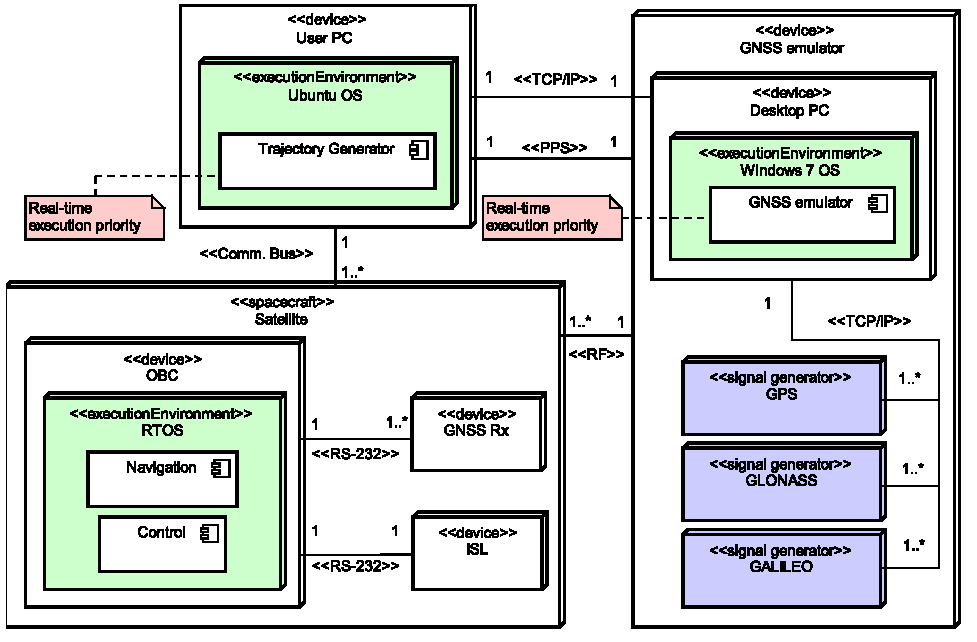
\includegraphics[scale=0.7]{media/main-body-chapter-results/fig-testbed-deployment-diagram-HIL.pdf}
	\caption{Testbed deployment.}\label{figure}
\end{figure}


\begin{lstlisting}[language=C++, style=StyleC, caption={Snippet}]
	typedef boost::interprocess::deque<Command, allocator_t> deque_t;
	typedef boost::interprocess::interprocess_mutex mutex_t;
	typedef boost::interprocess::scoped_lock<mutex_t> scoped_lock_t;
	typedef boost::interprocess::managed_shared_memory managed_shared_memory_t;
\end{lstlisting}

Nullam sed porta risus. Nulla non metus quis quam porta laoreet. Donec egestas nisl purus, a dignissim neque venenatis tempor. Proin facilisis quam eget sem vulputate ultrices. Aliquam sed enim id enim tincidunt sodales eget in enim. Nulla eget finibus libero. Fusce non tristique elit, eget varius erat. Pellentesque malesuada, nulla non rhoncus condimentum, leo nisi sagittis lacus, vel lobortis eros est pretium neque. Nulla nunc justo, convallis sed nibh sit amet, bibendum consectetur lacus.

\begin{lstlisting}[language=C++, style=StyleC,caption={Snippet: Definiciones de \texttt{TimeScale} y \texttt{TimeFormat} y comandos de control.},captionpos=b,label={defs_TimeScale_TimeFormat}]
	typedef enum TimeScale
	{
		UT1,
		UTC,
		TT,
		Uniform,
		InvalidTimeScale
	} TimeScale;
	
	typedef enum TimeFormat
	{
		Gregorian,
		MJD,
		ElapsedTime,
		InvalidTimeFormat
	} TimeFormat;
	
	try
	{
		boost::optional<ControlCommand> _command;
		_command = _queue->try_pop();
		if (_command)
		_currentCommand = *_command;
	}
	catch (const std::exception& e)
	{
		std::cerr << "ERROR: ContinuousThruster::getActuatorAcceleration(): " << e.what();
	}	
\end{lstlisting}

Nullam sed porta risus. Nulla non metus quis quam porta laoreet. Donec egestas nisl purus, a dignissim neque venenatis tempor. Proin facilisis quam eget sem vulputate ultrices. Aliquam sed enim id enim tincidunt sodales eget in enim. Nulla eget finibus libero. Fusce non tristique elit, eget varius erat. Pellentesque malesuada, nulla non rhoncus condimentum, leo nisi sagittis lacus, vel lobortis eros est pretium neque. Nulla nunc justo, convallis sed nibh sit amet, bibendum consectetur lacus.

\begin{lstlisting}[style=StyleC, caption={Snippet: Mi código en C++}]
	int main() {
		return 0; // Hola mundo
	}
\end{lstlisting}

Nullam sed porta risus. Nulla non metus quis quam porta laoreet. Donec egestas nisl purus, a dignissim neque venenatis tempor. Proin facilisis quam eget sem vulputate ultrices. Aliquam sed enim id enim tincidunt sodales eget in enim. Nulla eget finibus libero. Fusce non tristique elit, eget varius erat. Pellentesque malesuada, nulla non rhoncus condimentum, leo nisi sagittis lacus, vel lobortis eros est pretium neque. Nulla nunc justo, convallis sed nibh sit amet, bibendum consectetur lacus.

\begin{lstlisting}[language=yaml, caption={Snippet: Configuración YAML}]
	host: localhost
	port: 8080
\end{lstlisting}

Nullam sed porta risus. Nulla non metus quis quam porta laoreet. Donec egestas nisl purus, a dignissim neque venenatis tempor. Proin facilisis quam eget sem vulputate ultrices. Aliquam sed enim id enim tincidunt sodales eget in enim. Nulla eget finibus libero. Fusce non tristique elit, eget varius erat. Pellentesque malesuada, nulla non rhoncus condimentum, leo nisi sagittis lacus, vel lobortis eros est pretium neque. Nulla nunc justo, convallis sed nibh sit amet, bibendum consectetur lacus.

\begin{lstlisting}[style=terminal, caption={Vista desde una terminal Linux.}]
	$ g++ -Wall -pedantic main.cpp -o programa
	$ ./programa
	Hola Mundo!
\end{lstlisting}


\begin{algorithm}[t]
	\caption{Pseudocódigo del algoritmo AROM.}\label{alg_AROM}
	\begin{algorithmic}[1]
		\Require Posiciones y velocidades actuales de los satélites líder y seguidor.
		\Ensure  Comando de actuación.
		\Statex
		\Procedure{AROM}{}
		\Statex
		\State A partir de las posiciones y velocidades actuales del líder y seguidor, calcular sus elementos orbitales osculates $\xi_c$ y $\xi_d$, respectivamente, con $\xi = \left[a,\lambda_U,h_U,l_U,i,\Omega\right]^t$.
		\Statex
		\State Obtener los MOE $\bar{\xi}_c$ y $\bar{\xi}_d$ utilizando el algoritmo de Spiridonova con las perturbaciones.
		\Statex
		\State Calcular los MOE de la maniobra deseada actual como $\bar{\xi}_m(t) = \bar{\xi}_c + \delta_m^c\xi(t)$.
		\Statex
		\State Calcular el error MOE del seguidor respecto de la maniobra $\delta_d^m \bar{\xi} = \bar{\xi}_d - \bar{\xi}_m$, y del seguidor respecto del líder $\delta_d^c \bar{\xi} = \bar{\xi}_d - \bar{\xi}_c$.
		\Statex
		\State Etc..
		\Statex
		\EndProcedure
	\end{algorithmic}
\end{algorithm}

%% -------------------------------------
%%
%% Conclusions file.
%%
%% ---------------------
%% Change log:
%% 	2026-03-15 - initial version.
%%
%% ---------------------
%% Authors:
%% 	Santiago Husain Cerruti - hola dot santiago at proton dot me
%%
%% ---------------------
%% Filename: main-body-conclusions.tex
%% Part of FIUBA-thesis project.
%% Copyright (c) 2026 Santiago Husain Cerruti.
%% Licensed under the MIT License.
%% See LICENSE file for full text.
% -------------------------------------
\chapter{Conclusiones y trabajos futuros}

\hfill%
\begin{minipage}{0.7\textwidth}
	\begin{flushright}
		\emph{\enquote{The universe is a pretty big place. It’s bigger than anything anyone has ever dreamed of before. So if it’s just us...seems like an awful waste of space, right?}
			\vspace{5mm}}
		
		― Carl Sagan - Contact.
	\end{flushright}
\end{minipage}
\vspace{15mm}

Lorem ipsum dolor sit amet, consectetur adipiscing elit. Quisque semper arcu vel enim consectetur, facilisis feugiat dolor bibendum. Donec commodo lacus eget elit dapibus, a venenatis felis consequat. Aliquam consectetur lectus eu dui volutpat scelerisque. Sed laoreet nisi in magna eleifend tempus. Ut ac urna nec nunc tincidunt cursus sit amet eu purus. Sed convallis gravida mi, egestas finibus felis tempus vel. Donec odio sem, laoreet eget maximus elementum, commodo in mi. Pellentesque ut placerat ante. In eu justo eget ligula bibendum molestie eget in nulla. Nam malesuada nisl orci, elementum vulputate nisl pharetra sit amet. Nulla sit amet viverra tortor, a volutpat quam. Nulla quis mauris a justo consequat gravida. Donec posuere lorem id consectetur egestas.

Lorem ipsum dolor sit amet, consectetur adipiscing elit. Quisque semper arcu vel enim consectetur, facilisis feugiat dolor bibendum. Donec commodo lacus eget elit dapibus, a venenatis felis consequat. Aliquam consectetur lectus eu dui volutpat scelerisque. Sed laoreet nisi in magna eleifend tempus. Ut ac urna nec nunc tincidunt cursus sit amet eu purus. Sed convallis gravida mi, egestas finibus felis tempus vel. Donec odio sem, laoreet eget maximus elementum, commodo in mi. Pellentesque ut placerat ante. In eu justo eget ligula bibendum molestie eget in nulla. Nam malesuada nisl orci, elementum vulputate nisl pharetra sit amet. Nulla sit amet viverra tortor, a volutpat quam. Nulla quis mauris a justo consequat gravida. Donec posuere lorem id consectetur egestas.

% ---------------------------------------------------
% APPENDICES
% ---------------------------------------------------
\appendix
%% -------------------------------------
%%
%% Appendix page example file.
%%
%% ---------------------
%% Change log:
%% 	2026-03-15 - initial version.
%%
%% ---------------------
%% Authors:
%% 	Santiago Husain Cerruti - hola dot santiago at proton dot me
%%
%% ---------------------
%% Filename: back-matter-appendix-calculos-complementarios.tex
%% Part of FIUBA-thesis project.
%% Copyright (c) 2026 Santiago Husain Cerruti.
%% Licensed under the MIT License.
%% See LICENSE file for full text.
% -------------------------------------
\chapter{Cálculos complementarios}\label{appCalcMisc}

\section{Rotaciones elementales}
En el libro de \textcite{espana_book} se desarrollan las expresiones de rotaciones alrededor de los ejes de un sistema cartesiano, llamadas \emph{rotaciones elementales de Euler}. Si el ángulo a rotar es $\phi$, las expresiones de las matrices de rotación son las siguientes:

\begin{IEEEeqnarray}{rCl}
\mathbf{R}_x\left(\phi\right) & = &
\begin{bmatrix}
1 & 0 & 0 \\
0 & \cos \left(\phi\right) & \sin \left(\phi\right) \\
0 & -\sin \left(\phi\right) & \cos \left(\phi\right) \\
\end{bmatrix}
\end{IEEEeqnarray}

\begin{IEEEeqnarray}{rCl}
\mathbf{R}_y\left(\phi\right) & = &
\begin{bmatrix}
\cos \left(\phi\right) & 0 & -\sin \left(\phi\right) \\
0 & 1 & 0 \\
\sin \left(\phi\right) & 0 & \cos \left(\phi\right)\\
\end{bmatrix}
\end{IEEEeqnarray}

\begin{IEEEeqnarray}{rCl}
\mathbf{R}_z\left(\phi\right) & = &
	\begin{bmatrix}
	\cos \left(\phi\right) & \sin \left(\phi\right) & 0 \\
	-\sin \left(\phi\right) & \cos \left(\phi\right) & 0 \\
	0 & 0 & 1
	\end{bmatrix}
\end{IEEEeqnarray}


%% -------------------------------------
%%
%% Appendix page example file.
%%
%% ---------------------
%% Change log:
%% 	2026-03-15 - initial version.
%%
%% ---------------------
%% Authors:
%% 	Santiago Husain Cerruti - hola dot santiago at proton dot me
%%
%% ---------------------
%% Filename: back-matter-appendix-nutation-theory-coefficients.tex
%% Part of FIUBA-thesis project.
%% Copyright (c) 2026 Santiago Husain Cerruti.
%% Licensed under the MIT License.
%% See LICENSE file for full text.
% -------------------------------------
\chapter{Valores numéricos de modelos varios}\label{app_tables}

\begin{table}[!htb]
	\centering
	\tiny
	\caption{Primeros 40 coeficientes correspondientes a la Teoría de Nutación IAU-1980.}
	\resizebox{\textwidth}{!}{\begin{tabular}{cccccccccc}
		\toprule
		\multicolumn{1}{c}{Coeficiente} & \multicolumn{1}{c}{$p_l$} & \multicolumn{1}{c}{$p_l'$} & \multicolumn{1}{c}{$p_F$} & \multicolumn{1}{c}{$p_D$} & \multicolumn{1}{c}{$p_\Omega$} & \multicolumn{1}{c}{$\Delta \hat{\psi} \left[0.001''\right]$} & \multicolumn{1}{c}{$\Delta \hat{\psi}_T\left[0.001''\right]$} & \multicolumn{1}{c}{$\Delta \hat{\varepsilon}\left[0.001''\right]$} & \multicolumn{1}{c}{$\Delta \hat{\varepsilon}_T\left[0.001''\right]$} \\
		\midrule
		1     & 0     & 0     & 0     & 0     & 1     & -1719960 & -1742 & 920250 & 89 \\
		2     & 0     & 0     & 0     & 0     & 2     & 20620 & 2     & -8950 & 5 \\
		3     & -2    & 0     & 2     & 0     & 1     & 460   & 0     & -240  & 0 \\
		4     & 2     & 0     & -2    & 0     & 0     & 110   & 0     & 0     & 0 \\
		5     & -2    & 0     & 2     & 0     & 2     & -30   & 0     & 10    & 0 \\
		6     & 1     & -1    & 0     & -1    & 0     & -30   & 0     & 0     & 0 \\
		7     & 0     & -2    & 2     & -2    & 1     & -20   & 0     & 10    & 0 \\
		8     & 2     & 0     & -2    & 0     & 1     & 10    & 0     & 0     & 0 \\
		9     & 0     & 0     & 2     & -2    & 2     & -131870 & -16   & 57360 & -31 \\
		10    & 0     & 1     & 0     & 0     & 0     & 14260 & -34   & 540   & -1 \\
		11    & 0     & 1     & 2     & -2    & 2     & -5170 & 12    & 2240  & -6 \\
		12    & 0     & -1    & 2     & -2    & 2     & 2170  & -5    & -950  & 3 \\
		13    & 0     & 0     & 2     & -2    & 1     & 1290  & 1     & -700  & 0 \\
		14    & 2     & 0     & 0     & -2    & 0     & 480   & 0     & 10    & 0 \\
		15    & 0     & 0     & 2     & -2    & 0     & -220  & 0     & 0     & 0 \\
		16    & 0     & 2     & 0     & 0     & 0     & 170   & -1    & 0     & 0 \\
		17    & 0     & 1     & 0     & 0     & 1     & -150  & 0     & 90    & 0 \\
		18    & 0     & 2     & 2     & -2    & 2     & -160  & 1     & 70    & 0 \\
		19    & 0     & -1    & 0     & 0     & 1     & -120  & 0     & 60    & 0 \\
		20    & -2    & 0     & 0     & 2     & 1     & -60   & 0     & 30    & 0 \\
		21    & 0     & -1    & 2     & -2    & 1     & -50   & 0     & 30    & 0 \\
		22    & 2     & 0     & 0     & -2    & 1     & 40    & 0     & -20   & 0 \\
		23    & 0     & 1     & 2     & -2    & 1     & 40    & 0     & -20   & 0 \\
		24    & 1     & 0     & 0     & -1    & 0     & -40   & 0     & 0     & 0 \\
		25    & 2     & 1     & 0     & -2    & 0     & 10    & 0     & 0     & 0 \\
		26    & 0     & 0     & -2    & 2     & 1     & 10    & 0     & 0     & 0 \\
		27    & 0     & 1     & -2    & 2     & 0     & -10   & 0     & 0     & 0 \\
		28    & 0     & 1     & 0     & 0     & 2     & 10    & 0     & 0     & 0 \\
		29    & -1    & 0     & 0     & 1     & 1     & 10    & 0     & 0     & 0 \\
		30    & 0     & 1     & 2     & -2    & 0     & -10   & 0     & 0     & 0 \\
		31    & 0     & 0     & 2     & 0     & 2     & -22740 & -2    & 9770  & -5 \\
		32    & 1     & 0     & 0     & 0     & 0     & 7120  & 1     & -70   & 0 \\
		33    & 0     & 0     & 2     & 0     & 1     & -3860 & -4    & 2000  & 0 \\
		34    & 1     & 0     & 2     & 0     & 2     & -3010 & 0     & 1290  & -1 \\
		35    & 1     & 0     & 0     & -2    & 0     & -1580 & 0     & -10   & 0 \\
		36    & -1    & 0     & 2     & 0     & 2     & 1230  & 0     & -530  & 0 \\
		37    & 0     & 0     & 0     & 2     & 0     & 630   & 0     & -20   & 0 \\
		38    & 1     & 0     & 0     & 0     & 1     & 630   & 1     & -330  & 0 \\
		39    & -1    & 0     & 0     & 0     & 1     & -580  & -1    & 320   & 0 \\
		40    & -1    & 0     & 2     & 2     & 2     & -590  & 0     & 260   & 0 \\
		\bottomrule
	\end{tabular}}%
	\label{table:coefs_nut}
\end{table}%

\begin{table}[!htb]
	\centering
	\caption{Valores de densidades máxima y mínima para el modelo Harris-Priester en función de la altura sobre el elipsoide terrestre para actividades solares medias (150 SFU).}
	\begin{tabular}{ccc|ccc}
		\toprule
		\multicolumn{1}{c}{h $\left[\SI{}{\kilo\metre}\right]$} & \multicolumn{1}{c}{$\rho_m \left[\SI{}{\gram / \kilo\metre\cubed}\right]$} & \multicolumn{1}{c|}{$\rho_M \left[\SI{}{\gram / \kilo\metre\cubed}\right]$} & \multicolumn{1}{c}{h $\left[\SI{}{\kilo\metre}\right]$} & \multicolumn{1}{c}{$\rho_m \left[\SI{}{\gram / \kilo\metre\cubed}\right]$} & \multicolumn{1}{c}{$\rho_M \left[\SI{}{\gram / \kilo\metre\cubed}\right]$} \\
		\midrule
		100   & 497400 & 497400 & 420   & 1,558 & 5,684 \\
		120   & 24900 & 24900 & 440   & 1,091 & 4,355 \\
		130   & 8377  & 8710  & 460   & 0,7701 & 3,362 \\
		140   & 3899  & 4059  & 480   & 0,5474 & 2,612 \\
		150   & 2122  & 2215  & 500   & 0,3916 & 2,042 \\
		160   & 1263  & 1344  & 520   & 0,2819 & 1,605 \\
		170   & 800,8 & 875,8 & 540   & 0,2042 & 1,267 \\
		180   & 528,3 & 601   & 560   & 0,1488 & 1,005 \\
		190   & 361,7 & 429,7 & 580   & 0,1092 & 0,7997 \\
		200   & 255,7 & 316,2 & 600   & 0,0807 & 0,639 \\
		210   & 183,9 & 239,6 & 620   & 0,06012 & 0,5123 \\
		220   & 134,1 & 185,3 & 640   & 0,04519 & 0,4121 \\
		230   & 99,49 & 145,5 & 660   & 0,0343 & 0,3325 \\
		240   & 74,88 & 115,7 & 680   & 0,02632 & 0,2691 \\
		250   & 57,09 & 93,08 & 700   & 0,02043 & 0,2185 \\
		260   & 44,03 & 75,55 & 720   & 0,01607 & 0,1779 \\
		270   & 34,3  & 61,82 & 740   & 0,01281 & 0,1452 \\
		280   & 26,97 & 50,95 & 760   & 0,01036 & 0,119 \\
		290   & 21,39 & 42,26 & 780   & 0,008496 & 0,09776 \\
		300   & 17,08 & 35,26 & 800   & 0,007069 & 0,08059 \\
		320   & 10,99 & 25,11 & 840   & 0,00468 & 0,05741 \\
		340   & 7,214 & 18,19 & 880   & 0,0032 & 0,0421 \\
		360   & 4,824 & 13,37 & 920   & 0,00221 & 0,0313 \\
		380   & 3,274 & 9,955 & 960   & 0,00156 & 0,0236 \\
		400   & 2,249 & 7,492 & 1000  & 0,00115 & 0,0181 \\
		\bottomrule
	\end{tabular}%
\label{table_harris_priester}
\end{table}%

% ---------------------------------------------------
% BIBLIGRAPHY
% ---------------------------------------------------
% This command prints all the bibliographic entries, even if they were not cited in the text.
\nocite{*}
\clearpage
% Add the Bibliography to the Table of Contents and print it.
\printbibliography[heading=bibintoc,title={Referencias}]

% ---------------------------------------------------
% AUTHORSHIP DECLARATION
% ---------------------------------------------------
%% -------------------------------------
%%
%% Authorship declaration page file.
%%
%% ---------------------
%% Change log:
%% 	2026-03-15 - initial version.
%%
%% ---------------------
%% Authors:
%% 	Santiago Husain Cerruti - hola dot santiago at proton dot me
%%
%% ---------------------
%% Filename: back-matter-authorship-declaration.tex
%% Part of FIUBA-thesis project.
%% Copyright (c) 2026 Santiago Husain Cerruti.
%% Licensed under the MIT License.
%% See LICENSE file for full text.
% -------------------------------------
\thispagestyle{empty}
\null\vspace{\stretch {1}}
\section*{Declaración de autoría y originalidad del trabajo}
\begin{flushleft}

\textbf{DECLARO QUE:}

El trabajo desarrollado en la presente tesis de grado de Ingeniería Electrónica de la Universidad de Buenos Aires es obra del abajo firmante. Es un trabajo original e inédito, por lo tanto el contenido del mismo y su publicación no infringen derechos de propiedad intelectual, industrial, secreto comercial o cualquier otro derecho de terceros.\newline

\textbf{SI UTILIZÓ IA, ESPECIFICAR PARA QUÉ. ELIMINAR SI NO CORRESPONDE}:\newline
Durante la preparación de este trabajo, el autor utilizó [Nombre de la herramienta, ej. ChatGPT-4o] desarrollado por [Empresa, ej. OpenAI] para [especificar motivo, ej. la revisión gramatical y mejora del estilo de redacción]. Tras el uso de esta herramienta, el contenido fue revisado, editado y verificado meticulosamente por el autor, quien asume la responsabilidad total de la precisión y originalidad de los contenidos presentados en esta tesis.
\newline

Igualmente asumo, ante a la Universidad de Buenos Aires y ante cualquier otra instancia, la responsabilidad que pudiera derivarse en caso de plagio de contenidos en la tesis presentada, conforme al ordenamiento jurídico vigente.
\newline

\begin{flushright}
	NOMBRE COMPLETO AUTOR.
\end{flushright}
DD de MM de AAAA, Ciudad Autónoma de Buenos Aires, Argentina.\newline
\end{flushleft}

\vspace{\stretch{2}}\null
\end{document}

